\chapter{Re:VIEW を apache で動かす}
\label{chap:reviewOnApache}

「AWS上にRe:VIEW環境を構築する」
http://qiita.com/nanbuwks/items/da9136f1b6f789aaffcf

からの発展で、Re:VIEW を Web上で動かします。

「組版システムReVIEWでQiitaから同人誌原稿を作る」
http://qiita.com/nanbuwks/items/ad4ed8b7fbda846ba997

この仕組みを使ってQiitaにある記事を薄い本形式のPDFにするようにします。

\section{apache と PHP}
\label{sec:6-1}

apt{-}get install apache2
apt{-}get install libapache2{-}mod{-}php5

\section{DocumentRootにreview環境を展開}
\label{sec:6-2}

cd /var/www/html
review{-}init template
chown {-}R www{-}data:www{-}data *

\section{This account is currently not available.}
\label{sec:6-3}

コマンド実行でエラーが出たので/etc/passwdファイルの

として、www{-}dataでシェルログインできるようにします。

\begin{reviewemlist}
www{-}data:x:33:33:www{-}data:/var/www:/usr/sbin/nologin
\end{reviewemlist}

↓

\begin{reviewemlist}
www{-}data:x:33:33:www{-}data:/var/www:/bin/bash
\end{reviewemlist}

su {-} www{-}data

としてチェック。

・・・としていたのですが、ロケール設定だけの問題だったかも知れません。
現在は、ログオンシェルは /usr/sbin/nologin で運用しています。

\section{review環境を展開します。}
\label{sec:6-4}

review{-}init book

各種フォルダを作ります。

mkdir articles
mkdir template

\section{テンプレートを作ります。}
\label{sec:6-5}

\begin{reviewemlist}
cp book/config.yml template
cd template
vim config.yaml
\end{reviewemlist}

config.yamlを適当に書きます。

書籍タイトル、著者、表紙を作らない、などを指定しておくといいでしょう。

複数人で執筆するので、
Qiitaの1つの記事が1章というようになります。

なのでQiitaの記事は

1人目

\begin{reviewemlist}
\#\# 1人目の1章見出し
内容
\#\#\# 1人目の1{-}2章見出し
内容
\#\# 1人目の2章見出し
内容
\end{reviewemlist}

2人目

\begin{reviewemlist}
\#\# 2人目の1章見出し
内容
\#\#\# 2人目の1{-}2章見出し
内容
\#\# 2人目の2章見出し
内容
\end{reviewemlist}

3人目

\begin{reviewemlist}
・
・
・
\end{reviewemlist}

となりますが、これを

\begin{reviewemlist}
\#\# 1人目のタイトル
1人目の肩書、名前
\#\#\# 1人目の1章見出し
内容
\#\#\#\# 1人目の1{-}2章見出し
内容
\#\#\# 1人目の2章見出し
内容
\#\# 2人目のタイトル
2人目の肩書、名前
\#\#\# 2人目の1章見出し
内容
\#\#\#\# 2人目の1{-}2章見出し
内容
\#\#\# 2人目の2章見出し
内容
\#\# 3人目のタイトル
・
・
・
\end{reviewemlist}

とします。

なので、qiitaから取得したmarkdownは、見出しレベルを変更するスクリプトを通します。

\begin{reviewemlist}
sed "s/\textasciicircum{}\#/\#\#/"  qiita.md
\end{reviewemlist}

とすれば良いことになります。

qiita.mdはqiitaから取得したmarkdownです。qiitaからmarkdownを取得するにはwgetを使います。
こういったものも含めて、処理を行うシェルスクリプトを作ります。

\begin{reviewemlist}
\#\# cat qiitaget.sh
URL=`ruby {-}Ku ../../makeurl.rb`
echo \textdollar{}URL
cd images

wget \textdollar{}URL {-}k {-}H {-}r {-}l 1 {-}nH {-}nd {-}A png,PNG,jpg,JPG,jpeg,JPEG,html  {-}R txt
cd ..

rm qiita.md
wget \textdollar{}URL.md {-}O qiita.md
sed "s/\textasciicircum{}\#/\#\#/"  qiita.md \textbar{} ruby {-}Ku ../../qiitamd.rb \textbar{} ruby {-}Ku ../../texblock.rb \textbar{} ruby {-}Ku ../../texinline.rb   \textgreater{} temp.md
head {-}1 temp.md \textbar{} sed "s/\textasciicircum{}/\#/" \textgreater{} \textdollar{}1.md
ruby  ../../makeauthor.rb  \textgreater{}\textgreater{} \textdollar{}1.md
tail {-}n +2 temp.md \textgreater{}\textgreater{} \textdollar{}1.md
ruby ../../escapeincode.rb \textdollar{}1.md \textbar{} ruby ../../preprocess.rb \textbar{}  md2review \textbar{} ruby {-}Ku ../../scalemd.rb \textgreater{} \textdollar{}1.re
rake pdf
mv book.pdf \textdollar{}1.pdf

\end{reviewemlist}

この、qiitaget.shはPHPからコマンド実行関数で呼び出します。

\begin{reviewemlist}
\#\# cat compile.php
\textless{}html\textgreater{}
\textless{}head\textgreater{}
\textless{}meta charset="UTF{-}8"\textgreater{}
\textless{}title\textgreater{}qiita2review\textless{}/title\textgreater{}
\textless{}style type="text/css"\textgreater{}
body \{
  color: \#000;
  background{-}color: \#ffffff;
\}

pre \{
  padding: 1em;
  color: \#aaffaa;
  background{-}color: \#aaaaaa;
\}
\textless{}/style\textgreater{}
\textless{}/head\textgreater{}
\textless{}body\textgreater{}
\textless{}?php

\textdollar{}sectionName = \textdollar{}\textunderscore{}GET["section"];
?\textgreater{}
\textless{}h1\textgreater{}section \textless{}?php echo \textdollar{}sectionName; ?\textgreater{} compile\textless{}/h1\textgreater{}




\textless{}pre\textgreater{}
\textless{}?php
passthru("export LC\textunderscore{}CTYPE=en\textunderscore{}US.UTF{-}8; export LANG=en\textunderscore{}US.UTF{-}8; cd articles/".\textdollar{}sectionName." ; ../../qiitaget.sh ".\textdollar{}sectionName);


  ?\textgreater{}

\textless{}/pre\textgreater{}

\textless{}form action="\textless{}?php echo "articles/".\textdollar{}sectionName."/".\textdollar{}sectionName; ?\textgreater{}.pdf" METHOD="GET" \textgreater{}
\textless{}input type=submit value="View PDF"\textgreater{}
\textless{}/form\textgreater{}

\textless{}form action="make.php" METHOD="GET" \textgreater{}
\textless{}input type=hidden name=section value=\textless{}?php echo \textdollar{}sectionName; ?\textgreater{}\textgreater{}
\textless{}input type=submit value="return"\textgreater{}


\textless{}/form\textgreater{}
\textless{}/body\textgreater{}
\textless{}/html\textgreater{}

\end{reviewemlist}

他のphpファイル、qiitaget.shから呼び出す各種フィルタスクリプトを作ります。

\begin{reviewemlist}
(省略・・・他記事を参照して下さい)

\end{reviewemlist}

ファイルはwww{-}dataをオーナーにします。

\begin{reviewemlist}
\#\# chown {-}R www{-}data:www{-}data *

\end{reviewemlist}

ファイル一覧です

\begin{reviewemlist}
root@ip{-}172{-}30{-}0{-}222:/var/www/html\# ls {-}alh
total 80K
drwxr{-}xr{-}x 5 www{-}data www{-}data 4.0K Apr  6 14:03 .
drwxr{-}xr{-}x 3 root     root     4.0K Apr  6 13:58 ..
drwxr{-}xr{-}x 4 www{-}data www{-}data 4.0K Apr  6 13:48 articles
drwxr{-}xr{-}x 5 www{-}data www{-}data 4.0K Apr  5 20:07 book
{-}rw{-}r{-}{-}r{-}{-} 1 www{-}data www{-}data  803 Apr  5 03:48 compile.php
{-}rwxr{-}xr{-}x 1 www{-}data www{-}data  680 Apr  6 12:31 escapeincode.rb
{-}rw{-}r{-}{-}r{-}{-} 1 root     root      213 Apr  6 14:03 .htaccess
{-}rw{-}r{-}{-}r{-}{-} 1 www{-}data www{-}data 1.1K Apr  5 05:02 index.php
{-}rw{-}r{-}{-}r{-}{-} 1 www{-}data www{-}data  235 Apr  4 16:19 makeauthor.rb
{-}rw{-}r{-}{-}r{-}{-} 1 www{-}data www{-}data 1.4K Apr  5 20:18 make.php
{-}rw{-}r{-}{-}r{-}{-} 1 www{-}data www{-}data   87 Apr  5 03:28 makeurl.rb
{-}rw{-}r{-}{-}r{-}{-} 1 www{-}data www{-}data 1.2K Apr  5 05:11 new.php
{-}rwxr{-}xr{-}x 1 www{-}data www{-}data 2.0K Apr  5 19:11 preprocess.rb
{-}rwxrwxrwx 1 www{-}data www{-}data  536 Apr  6 12:58 qiitaget.sh
{-}rwxrwxrwx 1 www{-}data www{-}data  458 Apr  3 17:45 qiitamd.rb
{-}rwxrwxrwx 1 www{-}data www{-}data  222 Apr  4 13:41 scalemd.rb
{-}rwxr{-}xr{-}x 1 www{-}data www{-}data 1.4K Apr  6 09:11 slash2braceincode.rb
drwxr{-}xr{-}x 2 www{-}data www{-}data 4.0K Apr  4 18:23 template
{-}rwxrwxrwx 1 www{-}data www{-}data  286 Apr  4 12:20 texblock.rb
{-}rwxr{-}xr{-}x 1 www{-}data www{-}data 1.2K Apr  5 11:18 texinline.rb
\end{reviewemlist}

閲覧系は誰でも見せますが、登録系はbasic認証でアクセス制限をかけます。

\begin{reviewemlist}
\#\# cat .htaccess
\textless{}Files \textasciitilde{} "\textasciicircum{}\reviewbackslash{}.(htaccess\textbar{}htpasswd)\textdollar{}"\textgreater{}
deny from all
\textless{}/Files\textgreater{}
AuthUserFile /var/www/.htpasswd
AuthName "Please enter your ID and password"
AuthType Basic
order deny,allow
\textless{}Files new.php\textgreater{}
require valid{-}user
\textless{}/Files\textgreater{}
\end{reviewemlist}

作成したサイトです

\begin{reviewimage}
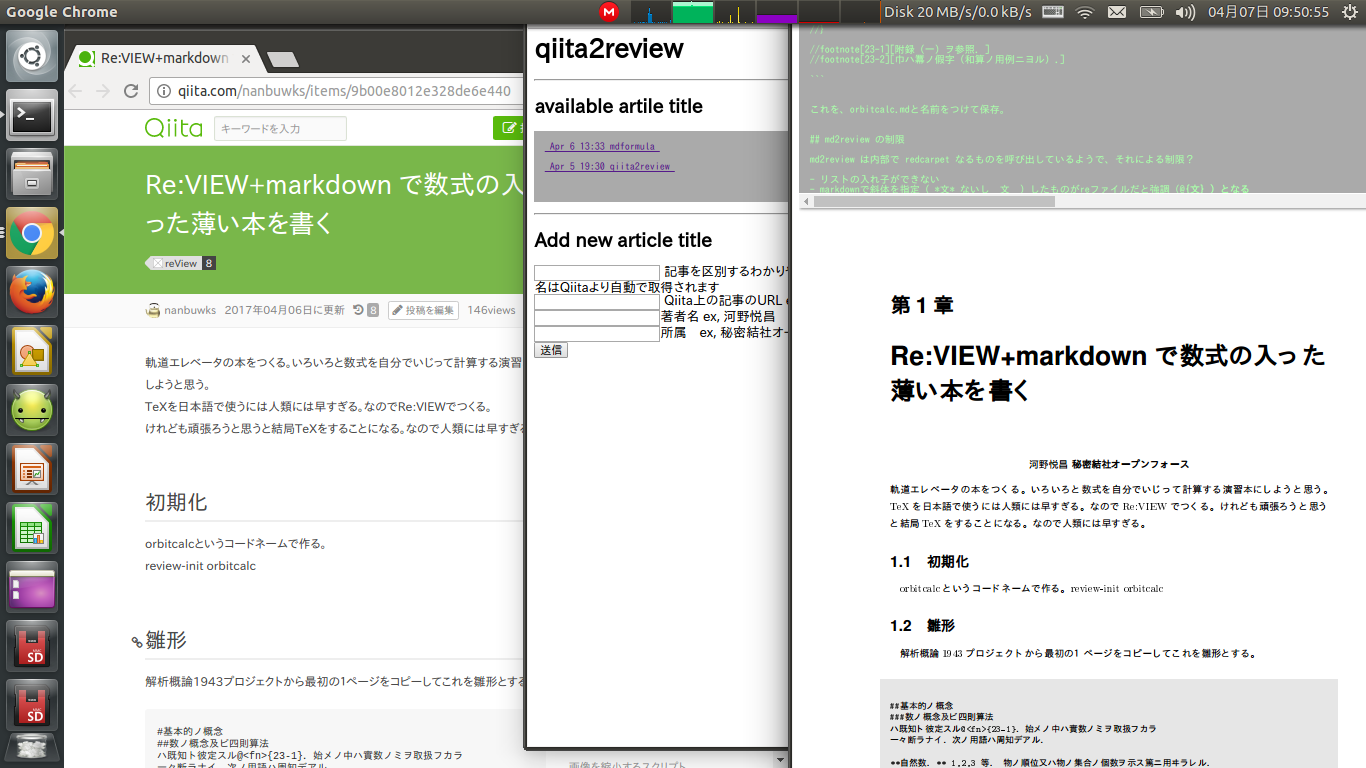
\includegraphics[width=\maxwidth]{./images/7b11276e-74ae-e25a-0872-3726cec353fb.png}
\caption{Screenshot from 2017{-}04{-}07 09{-}50{-}56.png}
\label{image:reviewOnApache:7b11276e-74ae-e25a-0872-3726cec353fb}
\end{reviewimage}
